\documentclass[12pt,letterpaper]{article}

%Note to Self:
%When Decommission? - after two months of feeling useless or right away?

\usepackage[utf8]{inputenc}
\usepackage[letterpaper,margin=1in]{geometry}
\usepackage{caption} % for table captions

\usepackage{amsmath} % for multi-line equations and piecewises
\usepackage{indentfirst} % to indent after a section
\usepackage{setspace}
\usepackage{times}
\usepackage{graphicx}
\usepackage{textcomp}
\usepackage{xspace}
\usepackage{verbatim} % for block comments
\usepackage{subfig} % for subfigures
\usepackage{enumitem} % for a) b) c) lists
\usepackage{tabularx}
\usepackage{cleveref}
\usepackage{xcolor}
\usepackage{soul}
\newcommand{\mathcolorbox}[2]{\colorbox{#1}{$\displaystyle #2$}}

\newcolumntype{b}{X}
\newcolumntype{s}{>{\hsize=.5\hsize}X}
\newcolumntype{m}{>{\hsize=.75\hsize}X}
\usepackage{titling}
\usepackage{minted}


\usepackage{tikz}


\usetikzlibrary{shapes.geometric,arrows}
\tikzstyle{process} = [rectangle, rounded corners, minimum width=3cm, minimum height=1cm,text centered, draw=black, fill=blue!30]
\tikzstyle{arrow} = [thick,->,>=stealth]


\graphicspath{{images/}}
 
\usepackage[font={footnotesize,it}]{caption}
 
\usepackage[toc,page]{appendix}


\setlength{\parindent}{15pt} % Default is 15pt.




\fontfamily{ptm}\selectfont

\title{CP2 for NPRE 501}
\author{Jin Whan Bae}
\date{2017-12-01}


\begin{document}
	
	\maketitle
	\hrule
	\onehalfspacing
	\thispagestyle{empty}

\section*{Problem Definition}

\Cref{tab:constants} lists the constants used in the problem.


\begin{table}[h]
     \centering
    \begin{tabular}{ccc}
       \hline
       Parameter & Value & [Unit] \\
       \hline
       \multicolumn{3}{c}{Thermal Hydraulic Data}\\
       \hline
       Inlet Temperature & 563 & K \\
       Outlet Temperature & 598 & K \\
       Inlet Velocity & 350 & cm/s \\
       System Pressure at Exit & 2200 & psi \\
       \hline
       \multicolumn{3}{c}{Assembly Data} \\
       \hline
       Clad Thickness & 0.0572 & cm \\
       Fuel-Pellet Diameter & 0.819 & cm \\
       Fuel Element Pitch & 1.25 & cm \\
       Fuel Element Outer Diameter & 0.94& cm \\
       Pellet-Clad Gap & 0.0082 & cm \\
       \textbf{Outer Radius} & 0.625 & cm \\
       \textbf{Total Fuel Radius} & 0.47 & cm \\
       \textbf{Active Core Height} & 366 & cm \\
       \hline
       \multicolumn{3}{c}{Assumed Constants - Avg at 580K} \\
       \hline
       Water Density & 0.6982 & $\frac{g}{cm^3}$ \\
       Specific Heat & 5.650 & $\frac{J}{g\cdot K}$ \\
       Thermal Conductivity ($UO_2$) & 0.4 \cite{ronchi_thermal_1999} & $\frac{J}{s\cdot m\cdot k}$ \\       
       \hline
    \end{tabular}
    \caption {Problem Constants.}
    \label{tab:constants}
\end{table}

From the constants, we can derive
\begin{table}[h]
     \centering
    \begin{tabular}{cccc}
    \hline
       Derived Constant & Equation & Value & Unit \\
    \hline
       Mass Flow & $ v * \rho * A $ & 130.29 & $\frac{g}{s}$ \\
    \hline
    \end{tabular}
    \caption {Derived Constants}
    \label{tab:der_constants}
\end{table}



\section* {1. Finding Heat Generation Rate}

The heat generation rate, given the inlet and outlet temperature
at steady-state conditions, can be found using this equation:

\[\int^{V} q'''(z) dV = C_p \dot{m} (T_{out} - T_{in})\]
\[[Area] \int^{L}_{0} q'''(z) dz = C_p \dot{m} (35 K)\]

\subsection*{Using a constant, average $C_p$ at 307.5C}
\[C_p \approx 5.650 \frac{J}{g K}\]

\[ \pi (0.47^2)  \int^{366}_{0} q'''(z) dz = 25766\]

Assuming $q'''(z) = C sin(\frac{\pi z}{L})$,
and L = 366cm:

\[ 0.6939 (366C(1-cos(\pi))) = 25766\]

\[161.69C = 25766\]
\[C = 159.34 \]

\[q'''(z) = 159.34 sin(\frac{\pi z}{L})\]

since q'(z) is $q'''(z) \cdot \pi R^2$:
\[q'(z) = 110.5 sin(\frac{\pi z}{L})\]

\subsection*{By Fitting an appropriately ordered polynomial}

The $C_p$ values are obtained using the IAPWS python
module \cite{romera_iapws:_2017}. The $C_p$ values
in the range are acquired and fitted using
the polyfit function in the numpy module.


The process of looking for an `appropriate' order fit was automated
by a python code (in appendix). The results are organized in table \ref{tab:poly_fit} as well as plotted in figure \ref{fig:poly_fit}.


\begin{table}[h]
     \centering
    \begin{tabular}{cc}
       \hline
       Order Fit & C Value  \\
       \hline
       1 & 163.67 \\
       2 & 164.1 \\
       3 & 164.19 \\
       4 & 164.22 \\
       5 & 164.22 \\
       \hline
    \end{tabular}
    \caption {Polynomial Fit Order and C Value.}
    \label{tab:poly_fit}
\end{table}


\begin{figure}[htbp!]
    \begin{center}
        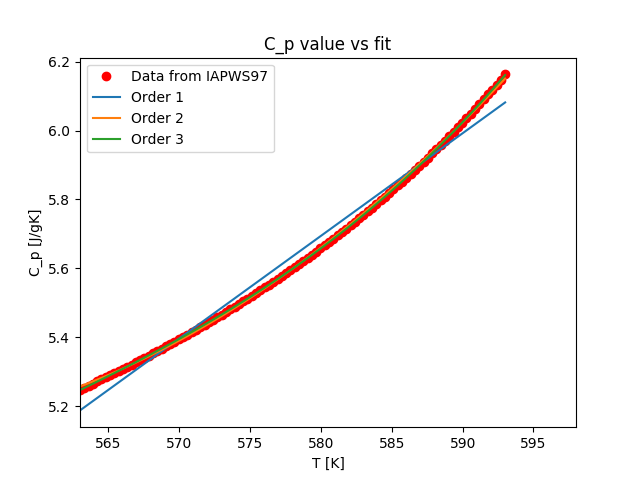
\includegraphics[scale=0.7]{cp_plot.png}
    \end{center}
    \caption{Temperature vs Heat Capacity from 563K to 598K}
    \label{fig:poly_fit}
\end{figure}


Considering the last three terms have little difference, we 
fit a second-order polynomial to obtain:

\[C_p = 4.67e-4T^2 -5.1e-1T + 144\]

Thus, using the second order polynomial fit, the volumetric
and linear heat generation becomes:

\[q'''(z) = 164.1 sin(\frac{\pi z}{L})\]
\[q'(z) = 113.8 sin(\frac{\pi z}{L})\]


\subsection*{Discuss.}
The answers to both a and b are quite similar, with minor differences.
The small difference may be due to the short temperature range where
the $C_p$ values are fitted. The little room for error is also reflected
on the almost-negligible change in the C value with change in the number of 
order fits. The volumetric heat generation with respect to height is plotted in
figure \ref{fig:q_vol}

\begin{figure}[htbp!]
    \begin{center}
        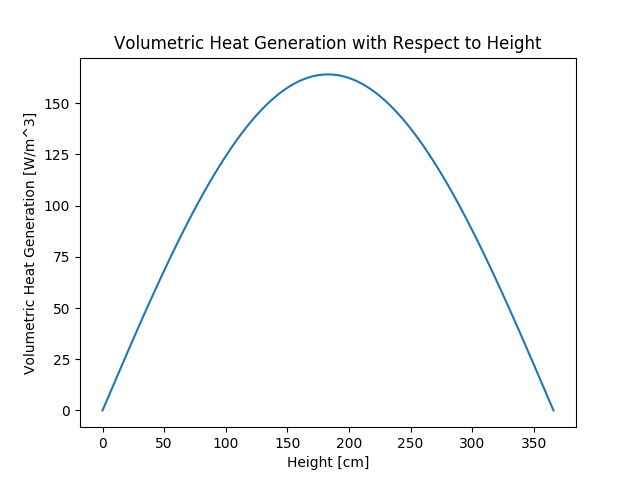
\includegraphics[scale=0.7]{q_vol_z.png}
    \end{center}
    \caption{Volumetric heat generation with respect to height obtained by polynomial fit.}
    \label{fig:q_vol}
\end{figure}




\section*{Coolant Temperature Profile}
With the heat generation found, it can be plugged back
into the energy equation to find $T_c(z)$:

\[[Area] \int^{z}_0 q'''(z) dz = \int^{T_c (z)}_{T_{in}} C_p(T) \dot{m} dT\]
\[\pi (.47^2) * 164.1 \int^{z}_0 sin(\frac{\pi z}{L})  dz =
    130.29 \int^{T_c (z)}_{T_{in}} (4.67e-4T^2 -5.1e-1T + 144)  dT\]
\[\pi (.47^2) * 164.1 * (\frac{L}{\pi} (1-cos(\frac{\pi z}{L}))) =
    130.29 (1.5e-4T^3 - .255T^2 + 144 T \Big{|}^{T_c (z)}_{T_{in}})\]

Putting numerical values instead of constants:

\[\pi (.47^2) * 164.1 * (\frac{366}{\pi} (1-cos(\frac{\pi z}{L}))) =
    130.29 (1.5e-4T^3 - .255T^2 + 144 T \Big{|}^{T_c (z)}_{563})\]

\[101.82 (1- cos(\frac{\pi z}{L})) + 27012 = 1.5e-4T_c^3 - .255T_c^2 + 144 T_c \]

\[-101.82 cos(\frac{\pi z}{L}) + 27114 = 1.5e-4T_c^3 - .255T_c^2 + 144 T_c \]

\[ cos(\frac{\pi z}{L}) = -1.47e-6T_c^3 + 0.0025T_c^2 -1.41 T_c + 265\]

To find $T_c(z)$, a root solver is used for every z value(code in appendix).
The coolant temperature profile is plotted in figure \ref{fig:t_c_z}.

\begin{figure}[htbp!]
    \begin{center}
        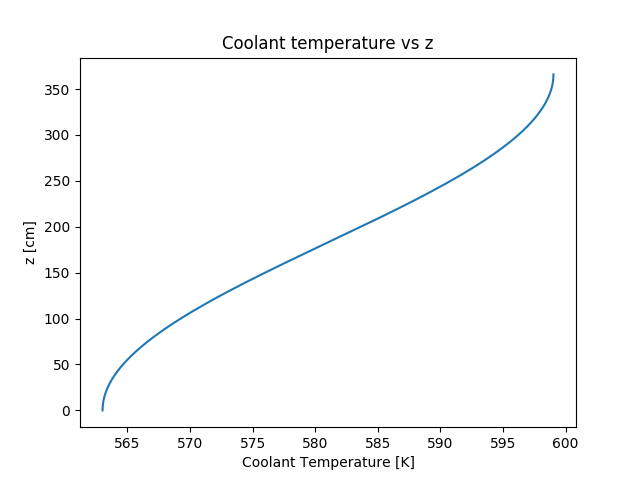
\includegraphics[scale=0.7]{t_c_z.png}
    \end{center}
    \caption{Temperature of coolant with respect to z.}
    \label{fig:t_c_z}
\end{figure}


\section*{Getting the heat transfer coefficient}
The heat transfer coefficient is obtained using the Dittus-Bolter Correlation,
where the Nusselt number is a function of the heat transfer coefficient.

\[ Nu = 0.023 Re^{0.8} Pr^{0.4} = \frac{h L}{k}\]

\[ Nu = 0.023 (\frac{\rho v L}{\mu})^{0.8} (\frac{\mu C_p}{k})^{0.4} = \frac{h L}{k}\]

where
\[v = \text{velocity of fluid} = 350 \frac{cm}{s}\]
\[L = \text{Characteristic length} = .31 cm \]
\[\rho = \text{Density of Fluid} \approx 0.7096 \frac{g}{cm^3}\]
\[\mu = \text{viscosity of fluid} \approx 0.00086 \frac{g}{cm s}\]
\[C_p = \text{ Specific Heat of fluid} \approx 5.650 \frac{J}{g K} \]
\[k = \text{thermal conductivity of fluid} \approx 0.00563\frac{W}{cm K} \]

the ones with $\approx$ are values that change with temperature. The temperature
for the approximate values are at 573K. Given this temperature, the Nusselt Number 
becomes 197.17, and heat transfer coefficient 3.5854 $\frac{W}{cm^2 K}$.

For different values of temperature given at different heights, the heat
transfer coefficient was calculated and plotted using a script (in appendix).
The plot is shown in figure \ref{fig:h_z}

\begin{figure}[htbp!]
    \begin{center}
        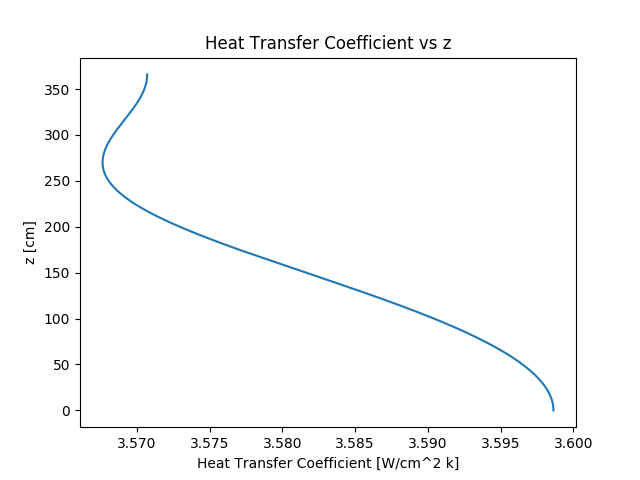
\includegraphics[scale=0.7]{h_z.png}
    \end{center}
    \caption{Heat Transfer Coefficient vs Z.}
    \label{fig:h_z}
\end{figure}

\section*{Using Computer Code for Temperature Distribution in Fuel Rod}

The temperature in the fuel rod is governed by the differential equation:
\[ \frac{d^2T}{dz^2} + \frac{1}{r} \frac{d}{dr} (r \frac{dT}{dr}) + \frac{q'''(z)}{k} = 0\]

\[ \frac{d^2T}{dz^2} + (\frac{d^2T}{dr^2} + \frac{1}{r} \frac{dT}{dr}) + \frac{q'''(z)}{k} = 0\]

Using the finite difference method, the differential equation becomes,

\[\frac{u_{z+1}^r - 2u_z^r + u_{z-1}}{dz^2}^r + \frac{u^{r+1}_z - 2u^r_z + u^{r-1}_z}{dr^2}
  + \frac{1}{r} \frac{u^{r+1}_z - u^{r-1}_z}{2dr} + \frac{q_z^r}{k} = 0 \]

solving for $u_z^r$:

\[ u_z^r = \frac{\frac{u_{z+1}^r + u_{z-1}^r}{dz^2} + \frac{u^{r+1}_z + u^{r-1}_z}{dr^2}
  + \frac{1}{r} \frac{u^{r+1}_z - u^{r-1}_z}{2dr} + \frac{q_z}{k}}{\frac{2}{dz^2} + \frac{2}{dr^2}} \]

With boundary conditions:

\begin{enumerate}
    \item $\frac{dT}{dr}(r=0) = 0$
    \item $-k \frac{dT}{dr} (r=R) = h(T(r=R) - T_c)$
    \item $\frac{dT}{dz}(z=0) = 0 $
    \item $\frac{dT}{dz}(z=L) = 0 $
\end{enumerate}

using finite difference, the boundary conditions become the following.
The first index is the z element, and the second the r element. The indexing
standard follows Python.
\begin{enumerate}
    \item $u[z][1]-u[z][0] = 0$
    \item $-k \frac{u[z][-2]-u[z][-1]}{dr} = h(u[z][-1] - T_c)$
    \item $ \frac{u[1][r] - u[0][r]}{dz} = 0$
    \item $\frac{u[-2][r] - u[-1][r]}{dz} = 0 $
\end{enumerate}

Using the finite difference approximations, and the boundary conditions,
the radial temperature profile is calculated (code in Appendix) and plotted in figure \ref{fig:numer}.
The temperature is highest at the center of the fuel (both radially
and axially) because the generated heat is retained. The L/2 and 3L/4 temperature are
similar in profile, but has minor difference in magnitude. Note the intersection of
L/2 and 3L/4, where the temperature drops faster at L/2 because the temperature gradient
is higher, and since the coolant temperature at 3L/4 is higher, there is less convective
cooling at the boundaries for 3L/4. 

\begin{figure}[htbp!]
    \begin{center}
        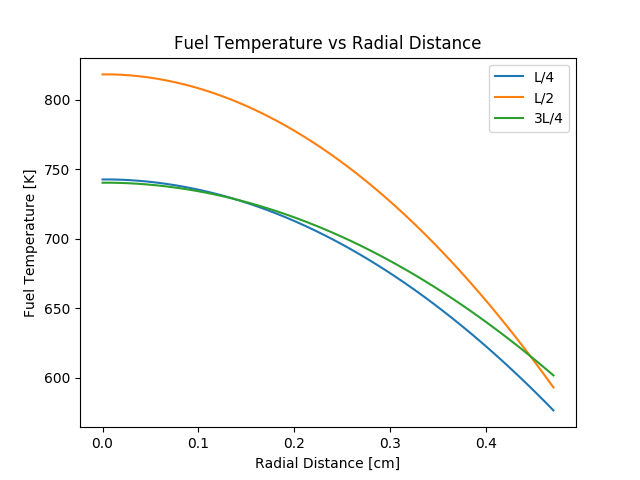
\includegraphics[scale=0.7]{numerical.png}
    \end{center}
    \caption{Temperature of Fuel with respect to r for different z values found using finite difference method.}
    \label{fig:numer}
\end{figure}


The temperature profile with respect to z given r = 0 is shown in figure \ref{fig:numer2}.
The temperature profile closely follows the heat generation profile, illustrated in
figure \ref{fig:q_vol}.


\begin{figure}[htbp!]
    \begin{center}
        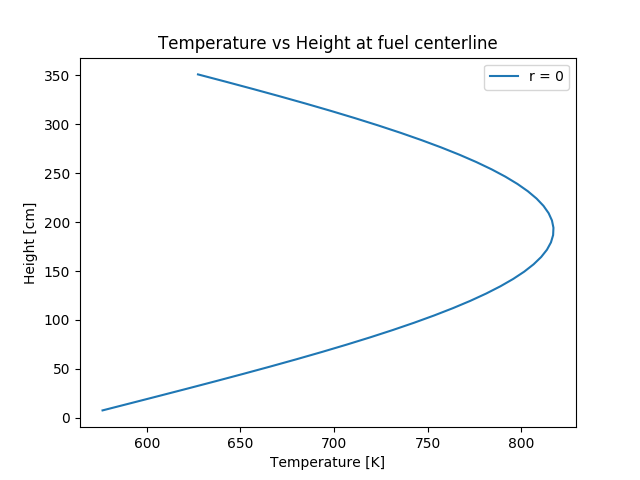
\includegraphics[scale=0.7]{fuel_centerline.png}
    \end{center}
    \caption{Temperature of Fuel centerline with respect to z calculated using finite difference method.}
    \label{fig:numer2}
\end{figure}


The temperature profile with respect to z given r = R and coolant temperature is shown
in figure \ref{fig:numer3}. Note the temperature at the fuel boundary is larger, intuitively
so, because heat flows from the fuel to the coolant. Note also the fuel boundary temperature
decreases towards the top, due to heat generation reduction.


\begin{figure}[htbp!]
    \begin{center}
        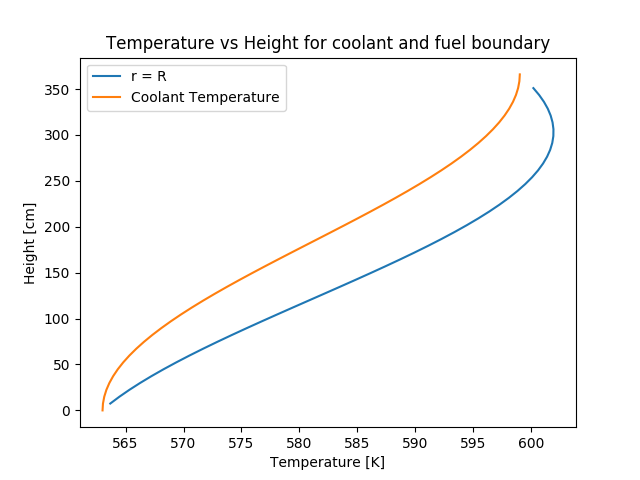
\includegraphics[scale=0.7]{fuel_bound.png}
    \end{center}
    \caption{Fuel boundary and coolant temperature with respect to z.}
    \label{fig:numer3}
\end{figure}

\pagebreak

\section*{Analytically Solve 1D Fuel Temperature Profile}
Ignoring Axial Conduction, we get:

\[\frac{1}{r} \frac{d}{dr} (r \frac{dT}{dr}) = \frac{-q'''(z)}{k}\]
\[k = 0.04 \frac{W}{cm\cdot K}\]

q'''(z) and $T_c$, and h  values for z values L/4, L/2, 3L/4 are listed in table \ref{tab:q_vol}.
The values are obtained from previous problems, and using a script (in appendix).


\begin{table}[h]
     \centering
    \begin{tabular}{cccc}
       \hline
       z value & q'''(z) [W/cmK] & $T_c(z) [K]$ & $h [\frac{W}{cm^2 K}] $ \\
       \hline
       L/4 & 116.03 & 568.2 & 3.591 \\
       L/2 & 164.1 & 581.04 & 3.575 \\
       3L/4 & 116.03 & 593.78 & 3.567 \\
       \hline
    \end{tabular}
    \caption {q'''(z), $T_c$ and h value for various z values}
    \label{tab:q_vol}
\end{table}

Integrating the differential equation to obtain the temperature profile for the
1D fuel:


\[ (r \frac{dT}{dr}) = \frac{-q'''(z)r^2}{2k} + C_1 \]

\[ \frac{dT}{dr} = \frac{-q'''(z)r}{2k} + \frac{C_1}{r} \]

\[ T_{1D} = \frac{-q'''(z)r^2}{4k} + C_1 ln(r) + C_2 \]
Applying BC at r=0, $C_1$ = 0.
Applying convective BC:
\[ -k \frac{dT}{dr}(r= 0.47 cm) = h (T(r = 0.47 cm ) - T_{coolant})\]
\[ -k( \frac{q''' (.47)}{2k}) = h (\frac{-q'''(.47)^2}{4k} + C_2 - T_{coolant})\]
This makes:
\[C_2 = \frac{-k}{h} ( \frac{-q''' (0.47)}{2k}) + \frac{q''' (.47^2)}{4k} + T_{coolant}\]

\[ T_{1D} = \frac{-q'''(z)r^2}{4k} + \frac{-k}{h} ( \frac{-q''' (0.47)}{2k}) + \frac{q''' (.47^2)}{4k} + T_{coolant}\]


The $C_2$ values obtained with the equation is listed in table \ref{tab:c2}.
The fuel temperature is plotted with the numerical solution in figure \ref{fig:num_anal}.

\begin{table}[h]
     \centering
    \begin{tabular}{ccc}
       \hline
       z value & $C_2$ & equation \\
       \hline
       L/4 & 323.6  & $T_{1D} = \frac{-q'''(z)r^2}{4k} + 736.0$ \\
       L/2 & 234.29 & $T_{1D} = \frac{-q'''(z)r^2}{4k} + 818.38$ \\
       3L/4 & 348.30 & $T_{1D} = \frac{-q'''(z)r^2}{4k} + 761.61$\\
       \hline
    \end{tabular}
    \caption {$C_2$ value for different z values}
    \label{tab:c2}
\end{table}


\begin{figure}[htbp!]
    \begin{center}
        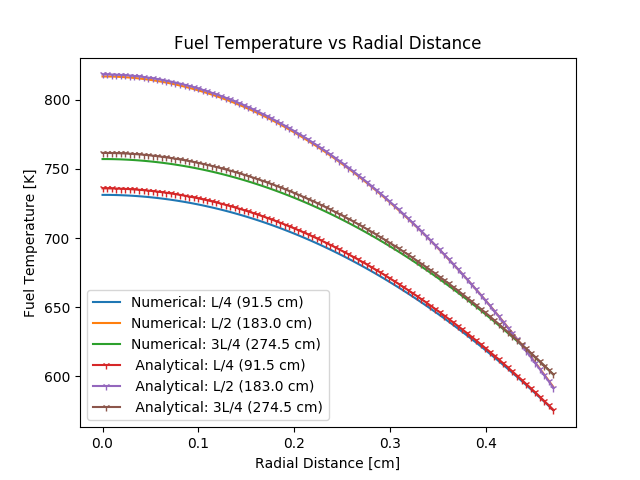
\includegraphics[scale=0.7]{num_anal.png}
    \end{center}
    \caption{Temperature of Fuel with respect to r for different z values obtained
             using both numerical and simplified analytical solution.}
    \label{fig:num_anal}
\end{figure}

The analytical solution obtained by ignoring axial conduction has
little difference with the numerical solution that takes into account
both axial and radial conduction, which means that axial conduction
has little role in the temperature distribution in the fuel, \textbf{if}
the two edges (top and bottom) are insulated. This again proves the importance
of setting an adequate boundary condition to solving differential equations.

\section*{Varying Density with Height}
Since temperature in the coolant varies with height in the core,
the density changes as well. The same module used to obtain $C_p$
is used to obtain the density values \cite{romera_iapws:_2017}.
For the range 563K to 598K, it follows a linear trend, as shown
in figure \ref{fig:wat_den}.  This gives an equation of:
\[\rho = -0.106T + 60.6384\]


\begin{figure}[htbp!]
    \begin{center}
        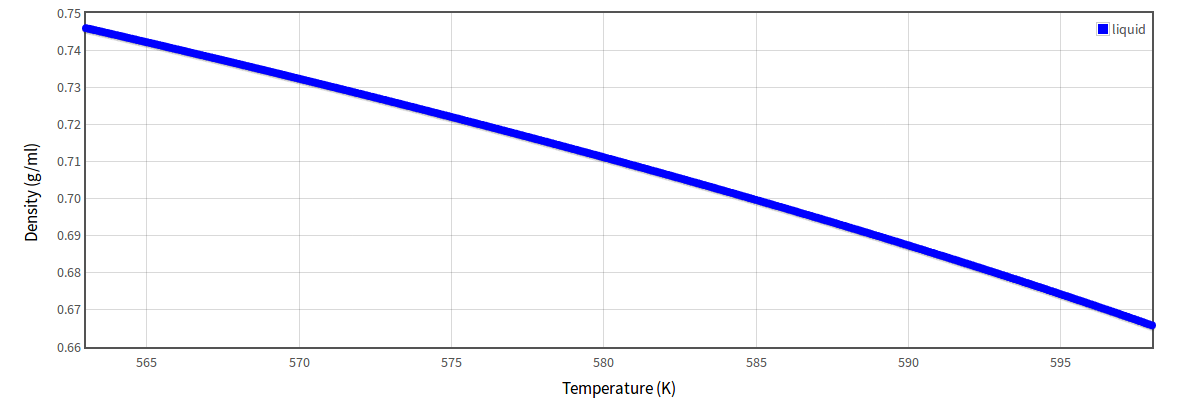
\includegraphics[scale=0.7]{water_density.png}
    \end{center}
    \caption{Density of water with respect to temperature, obtained from NIST \cite{acree_phase_?}.}
    \label{fig:wat_den}
\end{figure}

Plugging in the temperature value to obtain the density value
(code in Appendix), we get figure \ref{fig:rho_c_z}.

\begin{figure}[htbp!]
    \begin{center}
        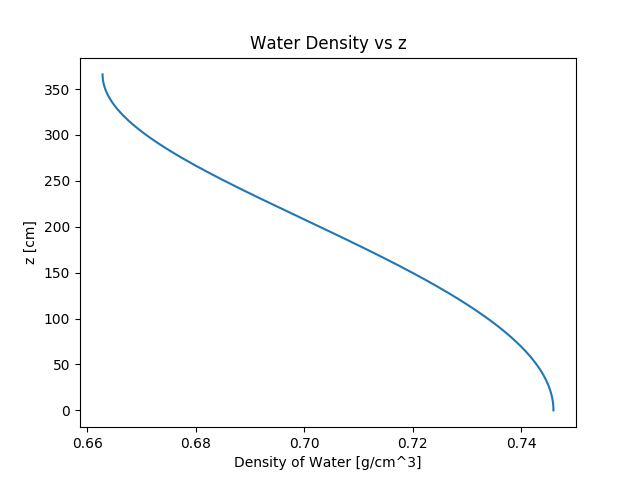
\includegraphics[scale=0.7]{rho_c_z.png}
    \end{center}
    \caption{Density of Coolant with respect to z.}
    \label{fig:rho_c_z}
\end{figure}

\section*{Varying Velocity with Height}
With the mass flow constant, the change in density
causes the change in velocity. The mass flow rate 
at the inlet is calculated with known temperature
563K, with density $0.7446 \frac{g}{cm^3}$.
An inlet mass flow rate is calculated by:
\[ \dot{m} = \rho(T) * u * A \]
\[ \dot{m} = 0.7446 * 350 * \pi * (0.625^2 - 0.47^2) \]
\[ \dot{m} = 0.7446 * 350 * \pi * (0.625^2 - 0.47^2) \]
\[ \dot{m} = 138.95 \frac{g}{s}\]

This is then kept constant and the u is varied by varying
density, caused by varying temperature.

\[ u = \frac{\dot{m}}{\rho * \pi * (0.625^2 - 0.47^2 )}\]

The flow velocity with respect to z is plotted using
a code (in appendix). The plot is shown in figure \ref{fig:u_c_z}.

\begin{figure}[htbp!]
    \begin{center}
        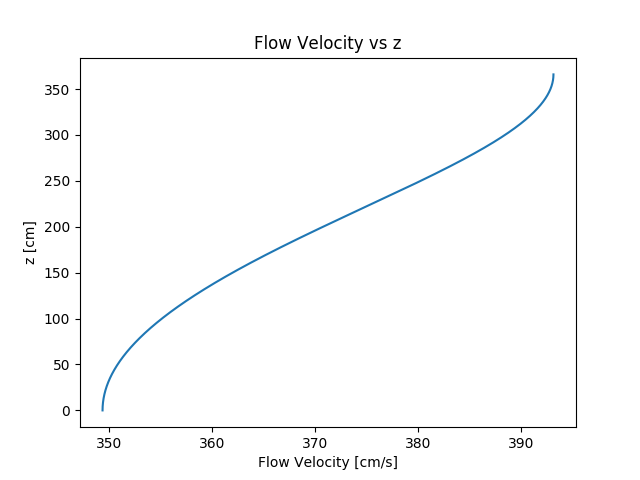
\includegraphics[scale=0.7]{u_c_z.png}
    \end{center}
    \caption{Flow velocity with respect to z.}
    \label{fig:u_c_z}
\end{figure}

\section*{Discussion of Ignoring Gap and Clad}
Ignoring the gap and clad allows a more efficient heat transfer
to the coolant, which leads to a lower fuel temperature. 
The gap has a low heat transfer coefficient, which `resists' heat
transfer from the fuel to the coolant, and leads to a higher
fuel temperature. Without the gap and the clad, the fuel is 
allowed to more efficiently be cooled by its direct contact
with the coolant, having a convective boundary condition with
the coolant directly. Thus the result from this computer project
does not reflect the reality correctly, due to its assumptions.



\pagebreak
\bibliographystyle{abbrv}
\bibliography{bibliography}
\pagebreak


\begin{appendices}

\section{For fitting polynomials for Heat Capacity}

\begin{minted}{python}
def fit_poly_cp(order):
    """ fits a polynomial for Temp and C_p of Water"""
    temp = np.linspace(290+273, 320+273, 100)
    cp =[]
    for i in temp:
        cp.append(IAPWS97(T=i, P=15.17).cp)
    eq = np.polyfit(temp, cp, order)
    eq = list(reversed(eq))
    x =np.polynomial.polynomial.Polynomial(eq)
    integral = integrate.quad(x, 290+273, 325+273)
    print('Result of the Integral for order %s is:' %str(order))
    print(integral[0])
    print('C = ')
    print(132.446*integral[0] / (366*2*.47**2))
    print('\n \n')
\end{minted}

\section{For finding $T_c(z)$}

\begin{minted}{python}
def root_solver():
    """ fits a polynomial for Temp and C_p of Water"""
    z = np.linspace(0, 366, 100)
    t_c = []
    for i in z:
        root = np.roots([-1.47e-6, 0.0025, -1.41, 276.23-np.cos(np.pi * i / 366)])
        print(root)
        print(type(root))
        filtered_root = float(str(root[0])[1:7])
        t_c.append(filtered_root)

    plt.plot(t_c, z)
    plt.show()
\end{minted}

\section{For finding h}

\begin{minted}{python}

def find_h():
    ri = 0.47
    ro = 0.625
    v = 350
    for i in [568.2, 581.04, 593.78]:
        L = 4 * np.pi*(ro**2 - ri**2) / (2*np.pi*ro + 2*np.pi*ri)
        mu = IAPWS97(T=i, P=15.17).mu * 10
        rho = IAPWS97(T=i, P=15.17).rho /1000
        cp = IAPWS97(T=i, P=15.17).cp
        k = IAPWS97(T=i, P=15.17).k /100
        Re = rho*v*L / mu
        Pr = mu*cp / k
        Nu = 0.023 * Re**(0.8) * Pr**(0.4)
        h = Nu * k / L
        print(h)
        print('\n')
\end{minted}

\section{Find}

\section{Numerical Method for finding Temperature Profile}
\begin{minted}{python}
def fuel_rod_temp(z_grid):
    """ temperature distribution in the fuel rod T_f(r,z)"""


    tol = 1e-3
    # k of UOX at 300C:
    k = 0.04 
    change = 10000
    z_list = np.linspace(0,366, z_grid)
    dz = z_list[1]-z_list[0]
    q_vol = 164.1*np.sin(np.pi * z_list / 366)
    r_list = np.linspace(0, 0.47, 100)
    dr = r_list[1]-r_list[0]
    h = find_h(z_grid)
    t_c = find_tc(z_grid)

    # 2d matrix with len(z) columns and len(r) rows
    t = np.zeros(shape=(len(z_list),len(r_list)), dtype=float)
    print(len(t))
    print(len(t[0]))
    # insulated bc at z=0 and z=L
    # convective bc at r = 0.47
    # r=0 bc

    trold = np.zeros(len(r_list))
    while True:
        told = np.copy(t)
        for z in range(1,len(z_list)-1):
            while True:
                tr = t[z][:]
                trold = tr.copy()
                for r in range(1,len(r_list)-1):
                    # z BC at the end
                    if z == len(z_list):
                        one = (2*t[z-1][r])/(dz**2)
                        two = (t[z][r+1] - t[z][r-1]) / (r_list[r] * 2*dr)
                        three = (t[z][r-1] + t[z][r+1]) / (dr**2)
                        four = q_vol[z] / k
                        denom = 2/(dz**2) + 2/(dr**2) 
                    # z BC at the beginning
                    elif z == 0:
                        one = (2*t[z+1][r])/(dz**2)
                        two = (t[z][r+1] - t[z][r-1]) / (r_list[r] * 2*dr)
                        three = (t[z][r-1] + t[z][r+1]) / (dr**2)
                        four = q_vol[z] / k
                        denom = 2/(dz**2) + 2/(dr**2) 
                    # all other scenarios
                    else:
                        one = (2*t[z+1][r])/(dz**2)
                        two = (t[z][r+1] - t[z][r-1]) / (r_list[r] * 2*dr)
                        three = (t[z][r-1] + t[z][r+1]) / (dr**2)
                        four = q_vol[z] / k
                        denom = 2/(dz**2) + 2/(dr**2) 

                    # do the addition to find t[z][r]
                    t[z][r] = (one + two + three + four) / denom
                # BC at r=0
                t[z][0] = t[z][1]
                #convective BC:
                t[z][-1] = (t[z][-2] + dr* (h[z]/k) * t_c[z]) / (1+ dr*h[z]/k)
                # (-h[z] * t_c[z] - (k*t[z][-2]/dr)) / (k/dr - h[z])
                conv = abs(tr-trold)
                if max(conv) < tol:
                    break

        conver = np.abs(t-told)
        if np.max(conver) < tol:
            break

    # constant z, varying r
    plt.plot(r_list, t[int(z_grid/4)], label='L/4 (%s cm)' %str(366/4))

    plt.plot(r_list, t[int(z_grid/2)], label='L/2 (%s cm)' %str(366/2))

    plt.plot(r_list, t[int(3*z_grid/4)], label='3L/4 (%s cm)' %str(3*366/4))
    plt.legend()
    plt.xlabel('Radial Distance [cm]')
    plt.ylabel('Fuel Temperature [K]')
    plt.title('Fuel Temperature vs Radial Distance')
    plt.savefig('numerical.png', format='png')
    plt.show()
    plt.close()


    # constant r, varying z
    plt.plot(t[:,0][1:-2], z_list[1:-2], label='r = 0')
    plt.plot(t[:,-1][1:-2], z_list[1:-2], label='r = R')
    plt.plot(t_c, z_list, label = 'Coolant Temperature')

    plt.legend()
    plt.xlabel('Temperature [K]')
    plt.ylabel('Height [cm]')
    plt.title('Temperature vs Height')
    plt.savefig('numerical2.png', format='png')
    plt.show()
    plt.close()

    # numerical and analytical together for varying r, constant z
    plt.plot(r_list, t[int(z_grid/4)], label='Numerical: L/4 (%s cm)' %str(366/4))
    plt.plot(r_list, t[int(z_grid/2)], label='Numerical: L/2 (%s cm)' %str(366/2))
    plt.plot(r_list, t[int(3*z_grid/4)], label='Numerical: 3L/4 (%s cm)' %str(3*366/4))

    R = 0.47
    k = 0.04
    L = 366
    q_vol_list = [116.03, 164.1, 116.03]
    h_list = [3.591, 3.575, 3.567]
    t_list = [568.22, 581.04, 593.78]
    L_list = [L/4, L/2, L*3/4]
    labels = ['L/4', 'L/2', '3L/4']
    for i in range(0, len(h_list)):
        c_2 = (k/h_list[i]) * (q_vol_list[i] * R / (2*k)) + q_vol_list[i] * (R**2)/(4*k) + t_list[i]
        r = np.linspace(0, 0.47, 100)
        print(c_2)
        t_r = (-q_vol_list[i]*r**2)/(4*k) + c_2
        plt.plot(r, t_r, marker='1', label= ' Analytical: ' + labels[i] + ' (' + str(L_list[i])[:5] + ' cm)')
    
    plt.legend()
    plt.xlabel('Radial Distance [cm]')
    plt.ylabel('Fuel Temperature [K]')
    plt.title('Fuel Temperature vs Radial Distance')
    plt.savefig('num_anal.png', format='png')
    plt.show()
    plt.close()

\end{minted}
\end{appendices}

\pagebreak

-end of report.
\end{document}






